% quadrature_decoder - quadrature decoder with or without clock input
% Written in 2016 by <Ahmet Inan> <xdsopl@googlemail.com>
% To the extent possible under law, the author(s) have dedicated all copyright and related and neighboring rights to this software to the public domain worldwide. This software is distributed without any warranty.
% You should have received a copy of the CC0 Public Domain Dedication along with this software. If not, see <http://creativecommons.org/publicdomain/zero/1.0/>.
\documentclass[a4paper]{article}
\usepackage{amsmath}
\usepackage{wrapfig}
\usepackage{gensymb}
\usepackage{hyperref}
\usepackage{fancyvrb}
\usepackage{tikz}
\usepackage{tikz-timing}
\usepackage[bottom]{footmisc}
\usetikzlibrary{circuits.logic.US}
\tikzstyle{branch}=[fill,shape=circle,minimum size=2pt,inner sep=0pt]
\title{Quadrature decoder with or without clock input\\- or -\\How to use a rotary encoder with an FPGA using VHDL}
\author{Ahmet Inan\\\href{mailto:xdsopl@googlemail.com}{\nolinkurl{xdsopl@googlemail.com}}}
\begin{document}
\maketitle
\begin{abstract}
It has been a long time since I played with 74HCT devices to build an 16-Bit-ISA card bus interface.
But times change and you wouldn't do that today having all these nice tools and devices.
I'm talking of course about CPLD (sea of gates) and FPGA (lookup tables) devices and most important of all, their design synthesis tools.
So I wanted to know, how rotary encoders work, how I could use them with FPGA's and also learn VHDL.
It's gonna be fun, let's go!
\end{abstract}
\begin{wrapfigure}{r}{0.5\textwidth}
\centering
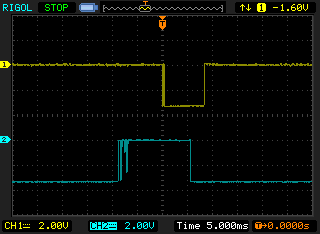
\includegraphics[width=0.5\textwidth]{quadrature_decoder_rigol.png}
\caption{Bounces caused by the mechanical switches of the rotary encoder}
\label{fig:bounces}
\end{wrapfigure}
\section{Contacts of mechanical switches bounce}
Before going to the logic operation side of things, let's first study the signals generated by a mechanical switch based rotary encoder.
As you can see from the signals captured~\footnote{Image created by Rigol DS1102E oscilloscope and inverted using ImageMagick \emph{convert}.}
by a dual channel oscilloscope in figure~\ref{fig:bounces},
the contacts of the mechanical switches inside of the rotary encoder will bounce while switching and create erratic pulses until they finally settle down.
Fortunately, only one of the two signals created by the rotary encoder will ever have those erratic pulses simultaneously.
So could we apply the things we've learned from debouncing a double throw switch with an SR~latch\footnote{Jack G. Ganssle wrote a very nice article about it: A Guide to Debouncing.}?
Yes, we can!
\newpage
\section{Quadrature signals}
Let's disregard the erratic pulses for a moment so we can focus on the interrelation of the signals shown in figure~\ref{fig:quadrature} created by a rotary encoder.
\begin{wrapfigure}{l}{0.5\textwidth}
\centering
\begin{tikztimingtable}
& SSS N(A1)SN(A2)SN(A3)SN(A4) SSS SSS SSS N(A5)SN(A6)SN(A7)SN(A8) SSS \\
$A$ & LLL HHL LLL SSS LLL LHH LLL \\
$B$ & LLL LHH LLL SSS LLL HHL LLL \\
& SSS N(B1)SN(B2)SN(B3)SN(B4) SSS SSS SSS N(B5)SN(B6)SN(B7)SN(B8) SSS \\
\extracode
\begin{pgfonlayer}{background}
\node at ($(A1)+(0,0.5)$) {\tiny$1$};
\node at ($(A2)+(0,0.5)$) {\tiny$2$};
\node at ($(A3)+(0,0.5)$) {\tiny$3$};
\node at ($(A4)+(0,0.5)$) {\tiny$4$};
\node at ($(A5)+(0,0.5)$) {\tiny$5$};
\node at ($(A6)+(0,0.5)$) {\tiny$6$};
\node at ($(A7)+(0,0.5)$) {\tiny$7$};
\node at ($(A8)+(0,0.5)$) {\tiny$8$};
\draw[help lines] (A1) -- (B1);
\draw[help lines] (A2) -- (B2);
\draw[help lines] (A3) -- (B3);
\draw[help lines] (A4) -- (B4);
\draw[help lines] (A5) -- (B5);
\draw[help lines] (A6) -- (B6);
\draw[help lines] (A7) -- (B7);
\draw[help lines] (A8) -- (B8);
\end{pgfonlayer}
\end{tikztimingtable}
\caption{Signals in quadrature}
\label{fig:quadrature}
\end{wrapfigure}
On the left you can see waveforms that happen when the wheel of the rotary encoder is turned one step left and one step right is what you see on the right side.
These signals are said to be \emph{in quadrature} as their relation is that they are ortogonal to each other or in simpler terms, $90\degree$ out of phase.
We can also gather, that there are only four signal level constellations we have to consider and creating the signals to be debounced by our trusty SR~latches is now easy:
\begin{align}
1-2, 7-8 &:& A = H &\land B = L &\implies& E \gets A \land \neg B\\
2-3, 6-7 &:& A = H &\land B = H &\implies& C \gets A \land B\\
3-4, 5-6 &:& A = L &\land B = H &\implies& F \gets B \land \neg A\\
    else &:& A = L &\land B = L &\implies& D \gets \neg (A \lor B)
\end{align}
\section{Design with logic gates}
Putting those new signals $C-F$ to good use and designing a circuit made from logic gates should lead us to something like shown in figure~\ref{fig:logic}.
\begin{figure}[h]
\centering
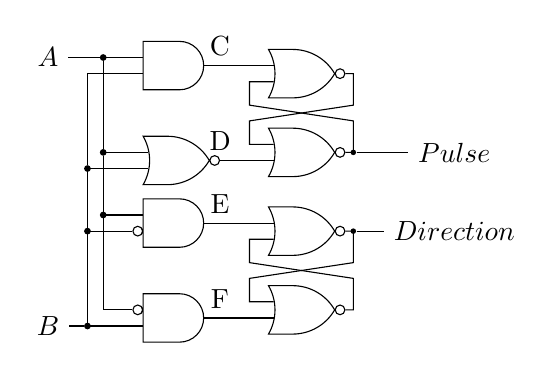
\begin{tikzpicture}[circuit logic US]
\node[nor gate, draw, inputs=nn] at (3,0) (Nor2) {};
\node[nor gate, draw, inputs=nn] at (3,1) (Nor3) {};
\node[nor gate, draw, inputs=nn] at (3,2) (Nor4) {};
\node[nor gate, draw, inputs=nn] at (3,3) (Nor5) {};
\node[and gate, draw, inputs=ni] at ($(Nor3.input 1)+(-1.3,0)$) (And1) {};
\node[and gate, draw, inputs=in] at ($(Nor2.input 2)+(-1.3,0)$) (And2) {};
\node[and gate, draw, inputs=nn] at ($(Nor5.input 1)+(-1.3,0)$) (And3) {};
\node[nor gate, draw, inputs=nn] at ($(Nor4.input 2)+(-1.3,0)$) (Nor1) {};
\node[branch, draw] at ($(And3.input 1)+(-0.5,0)$) (A1) {};
\node[branch, draw] at ($(A1 |- Nor1.input 1)$) (A2) {};
\node[branch, draw] at ($(A1 |- And1.input 1)$) (A3) {};
\node[branch, draw] at ($(And2.input 2)+(-0.7,0)$) (B1) {};
\node[branch, draw] at ($(B1 |- And1.input 2)$) (B2) {};
\node[branch, draw] at ($(B1 |- Nor1.input 2)$) (B3) {};
\node (A) at ($(A1)+(-0.7,0)$) {$A$};
\node (B) at ($(B1)+(-0.5,0)$) {$B$};
\node (P) at ($(Nor4)+(2,0)$) {$Pulse$};
\node (D) at ($(Nor3)+(2,0)$) {$Direction$};
\draw (A) -- (A1);
\draw (B) -- (B1);
\draw (A1) -- (A2);
\draw (A2) -- (A3);
\draw (B1) -- (B2);
\draw (B2) -- (B3);
\draw (A3) |- (And1.input 1);
\draw (B2) |- (And1.input 2);
\draw (A3) |- (And2.input 1);
\draw (B1) |- (And2.input 2);
\draw (A1) |- (And3.input 1);
\draw (B3) |- (And3.input 2);
\draw (A2) |- (Nor1.input 1);
\draw (B3) |- (Nor1.input 2);
\draw (And1.output) -- +(0.2,0) node[above]{E} -- (Nor3.input 1);
\draw (And2.output) -- +(0.2,0) node[above]{F} -- (Nor2.input 2);
\draw (Nor3.output) -| node[branch] (D1) {} +(0.1,-0.4) -- ($(Nor2)+(-0.6,+0.4)$) |- (Nor2.input 1);
\draw (Nor2.output) -| +(0.1,0.4) -- ($(Nor3)+(-0.6,-0.4)$) |- (Nor3.input 2);
\draw (D1) -- (D);
\draw (And3.output) -- +(0.2,0) node[above]{C} -- (Nor5.input 1);
\draw (Nor1.output) -- +(0,0) node[above]{D} -- (Nor4.input 2);
\draw (Nor5.output) -| +(0.1,-0.4) -- ($(Nor4)+(-0.6,+0.4)$) |- (Nor4.input 1);
\draw (Nor4.output) -| node[branch] (P1) {} +(0.1,0.4) -- ($(Nor5)+(-0.6,-0.4)$) |- (Nor5.input 2);
\draw (P1) -- (P);
\end{tikzpicture}
\caption{Logic gate circuit}
\label{fig:logic}
\end{figure}
\section{Understanding the circuit}
Analysing the waveforms of the signals $C$ to $F$, $Pulse$ and $Direction$ created by the circuit when stimulated by the clean signals $A$ and $B$ might look like in figure~\ref{fig:waveforms}.
\begin{figure}
\centering
\begin{tikztimingtable}
$A$         & LLL N(A1)HHN(A2)L LLL LN(A3)HHN(A4) LLL \\
$B$         & LLL LN(B1)HHN(B2) LLL N(B3)HHN(B4)L LLL \\
$C$         & LLL LN(C1)HN(C2)L LLL LN(C3)HN(C4)L LLL \\
$D$         & HHH N(D1)LLLN(D2) HHH N(D3)LLLN(D4) HHH \\
$E$         & LLL N(E1)HN(E2)LL LLL LLN(E3)HN(E4) LLL \\
$F$         & LLL LLN(F1)HN(F2) LLL N(F3)HN(F4)LL LLL \\
$Pulse$     & LLL LN(P1)HHN(P2) LLL LN(P3)HHN(P4) LLL \\
$Direction$ & LLL LLN(D1)H HHH HHN(D2)L LLL \\
\extracode
\begin{pgfonlayer}{background}
\draw[help lines] (A1) -- (E1);
\draw[help lines] (A2) -- (D1);
\draw[help lines] (A3) -- (P3);
\draw[help lines] (A4) -- (P4);
\draw[help lines] (B1) -- (P1);
\draw[help lines] (B2) -- (P2);
\draw[help lines] (B3) -- (F3);
\draw[help lines] (B4) -- (D2);
\end{pgfonlayer}
\end{tikztimingtable}
\caption{Clean waveforms}
\label{fig:waveforms}
\end{figure}
\newpage
\begin{figure}
\centering
\begin{BVerbatim}
c <= a and b;
d <= a nor b;
e <= a and not b;
f <= b and not a;
dir <= dir_n nor e;
dir_n <= dir nor f;
pul <= pul_n nor d;
pul_n <= pul nor c;
pulse <= pul;
direction <= dir;
\end{BVerbatim}
\caption{VHDL code of asynchronous design}
\end{figure}
\begin{figure}
\centering
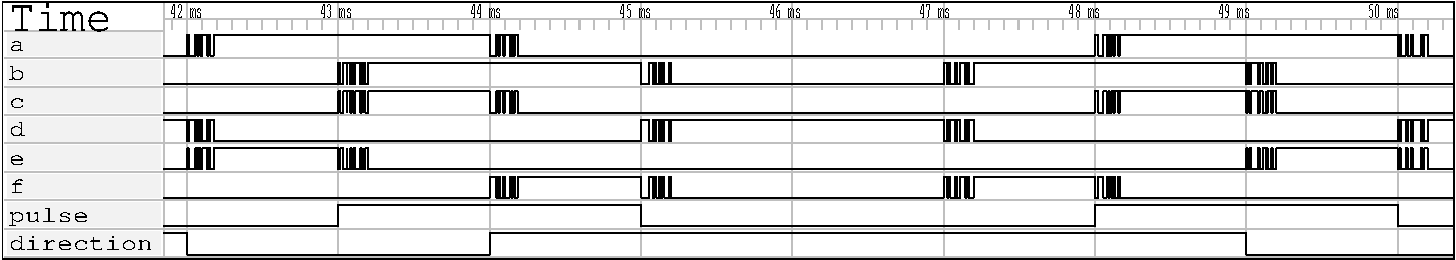
\includegraphics[width=\textwidth]{asynchronous_quadrature_decoder_gtkwave.pdf}
\caption{Waveforms of asynchronous design}
\end{figure}
\begin{figure}
\centering
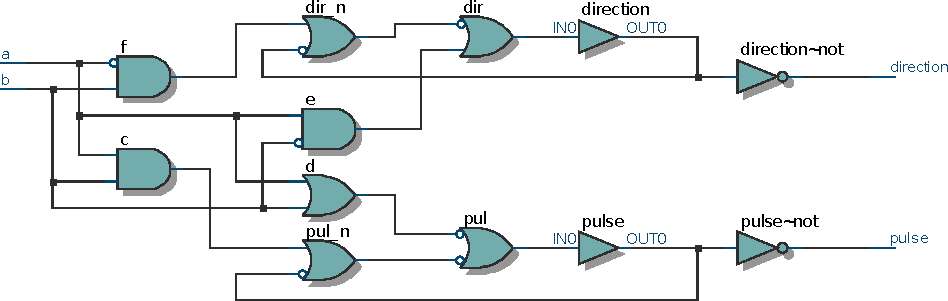
\includegraphics[width=0.5\textwidth]{asynchronous_quadrature_decoder_quartus_rtl.pdf}
\caption{RTL view of asynchronous design}
\end{figure}
\begin{figure}
\centering
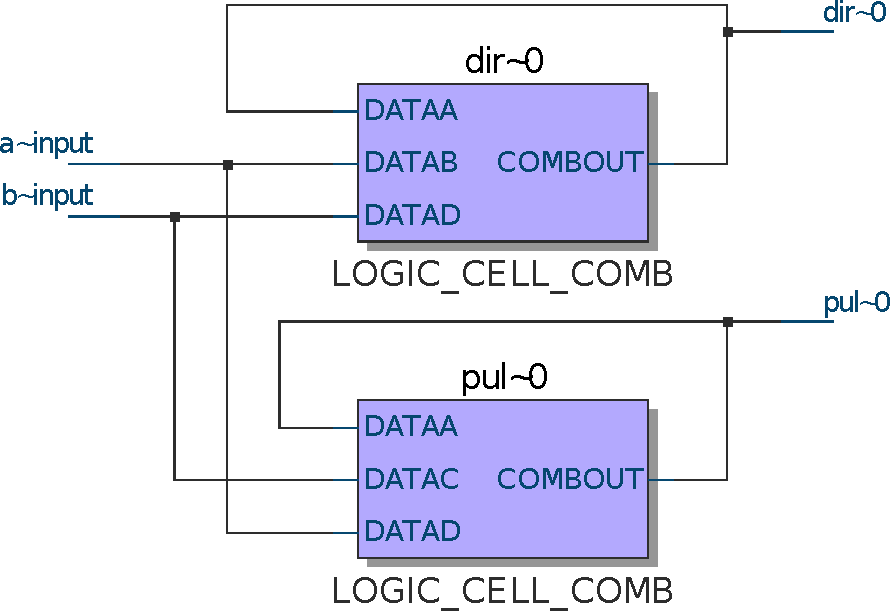
\includegraphics[width=0.5\textwidth]{asynchronous_quadrature_decoder_quartus_map.pdf}
\caption{Reduced to two combinational loops}
\end{figure}
\begin{figure}
\centering
\begin{BVerbatim}
Warning: Found combinational loop of 2 nodes
Warning (332126): Node "decoder_inst|pul~0|dataa"
Warning (332126): Node "decoder_inst|pul~0|combout"
Warning: Found combinational loop of 2 nodes
Warning (332126): Node "decoder_inst|dir~0|dataa"
Warning (332126): Node "decoder_inst|dir~0|combout"
\end{BVerbatim}
\caption{Combinational loop warning}
\end{figure}
\begin{figure}
\centering
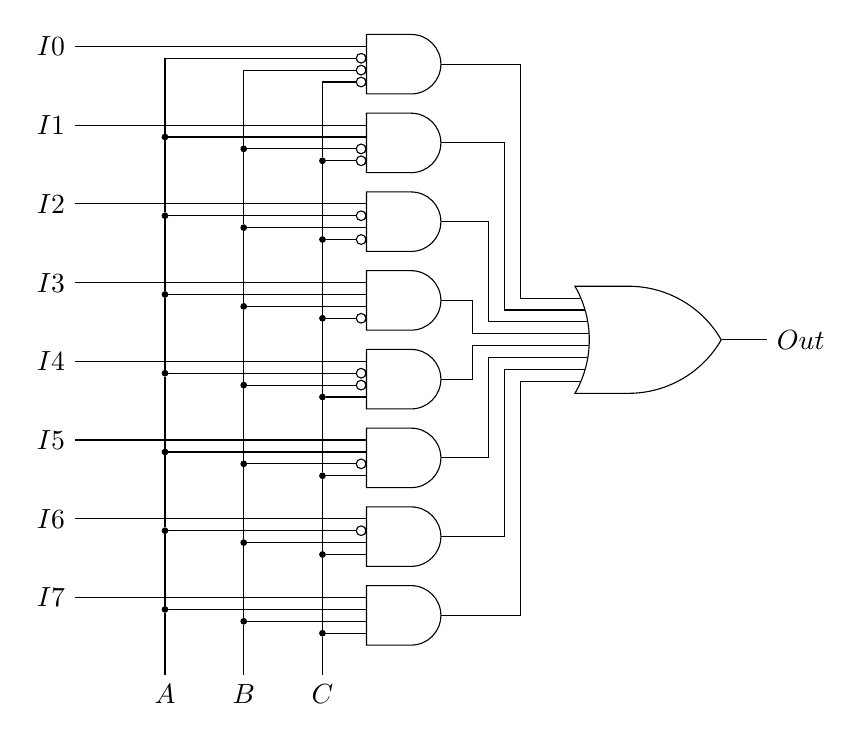
\begin{tikzpicture}[circuit logic US]
\node (A) at (1,0) {$A$};
\node (B) at (2,0) {$B$};
\node (C) at (3,0) {$C$};
\node[and gate, draw, inputs=niii] at (4,8) (And0) {};
\node[and gate, draw, inputs=nnii] at (4,7) (And1) {};
\node[and gate, draw, inputs=nini] at (4,6) (And2) {};
\node[and gate, draw, inputs=nnni] at (4,5) (And3) {};
\node[and gate, draw, inputs=niin] at (4,4) (And4) {};
\node[and gate, draw, inputs=nnin] at (4,3) (And5) {};
\node[and gate, draw, inputs=ninn] at (4,2) (And6) {};
\node[and gate, draw, inputs=nnnn] at (4,1) (And7) {};
\node[or gate, draw, inputs=nnnnnnnn] at (7,4.5) (Or0) {};
\node (O) at ($(Or0.output)+(1,0)$) {$Out$};
\node (I0) at ($(And0.input 1)+(-4,0)$) {$I0$};
\node (I1) at ($(And1.input 1)+(-4,0)$) {$I1$};
\node (I2) at ($(And2.input 1)+(-4,0)$) {$I2$};
\node (I3) at ($(And3.input 1)+(-4,0)$) {$I3$};
\node (I4) at ($(And4.input 1)+(-4,0)$) {$I4$};
\node (I5) at ($(And5.input 1)+(-4,0)$) {$I5$};
\node (I6) at ($(And6.input 1)+(-4,0)$) {$I6$};
\node (I7) at ($(And7.input 1)+(-4,0)$) {$I7$};
\node[branch, draw] at ($(And1.input 2 -| A)$) (A1) {};
\node[branch, draw] at ($(And1.input 3 -| B)$) (B1) {};
\node[branch, draw] at ($(And1.input 4 -| C)$) (C1) {};
\node[branch, draw] at ($(And2.input 2 -| A)$) (A2) {};
\node[branch, draw] at ($(And2.input 3 -| B)$) (B2) {};
\node[branch, draw] at ($(And2.input 4 -| C)$) (C2) {};
\node[branch, draw] at ($(And3.input 2 -| A)$) (A3) {};
\node[branch, draw] at ($(And3.input 3 -| B)$) (B3) {};
\node[branch, draw] at ($(And3.input 4 -| C)$) (C3) {};
\node[branch, draw] at ($(And4.input 2 -| A)$) (A4) {};
\node[branch, draw] at ($(And4.input 3 -| B)$) (B4) {};
\node[branch, draw] at ($(And4.input 4 -| C)$) (C4) {};
\node[branch, draw] at ($(And5.input 2 -| A)$) (A5) {};
\node[branch, draw] at ($(And5.input 3 -| B)$) (B5) {};
\node[branch, draw] at ($(And5.input 4 -| C)$) (C5) {};
\node[branch, draw] at ($(And6.input 2 -| A)$) (A6) {};
\node[branch, draw] at ($(And6.input 3 -| B)$) (B6) {};
\node[branch, draw] at ($(And6.input 4 -| C)$) (C6) {};
\node[branch, draw] at ($(And7.input 2 -| A)$) (A7) {};
\node[branch, draw] at ($(And7.input 3 -| B)$) (B7) {};
\node[branch, draw] at ($(And7.input 4 -| C)$) (C7) {};
\draw (I0) -- (And0.input 1);
\draw (I1) -- (And1.input 1);
\draw (I2) -- (And2.input 1);
\draw (I3) -- (And3.input 1);
\draw (I4) -- (And4.input 1);
\draw (I5) -- (And5.input 1);
\draw (I6) -- (And6.input 1);
\draw (I7) -- (And7.input 1);
\draw (A1) |- (And0.input 2);
\draw (B1) |- (And0.input 3);
\draw (C1) |- (And0.input 4);
\draw (A1) -- (And1.input 2);
\draw (B1) -- (And1.input 3);
\draw (C1) -- (And1.input 4);
\draw (A2) -- (And2.input 2);
\draw (B2) -- (And2.input 3);
\draw (C2) -- (And2.input 4);
\draw (A3) -- (And3.input 2);
\draw (B3) -- (And3.input 3);
\draw (C3) -- (And3.input 4);
\draw (A4) -- (And4.input 2);
\draw (B4) -- (And4.input 3);
\draw (C4) -- (And4.input 4);
\draw (A5) -- (And5.input 2);
\draw (B5) -- (And5.input 3);
\draw (C5) -- (And5.input 4);
\draw (A6) -- (And6.input 2);
\draw (B6) -- (And6.input 3);
\draw (C6) -- (And6.input 4);
\draw (A7) -- (And7.input 2);
\draw (B7) -- (And7.input 3);
\draw (C7) -- (And7.input 4);
\draw (A) -- (A7);
\draw (B) -- (B7);
\draw (C) -- (C7);
\draw (A1) -- (A2);
\draw (B1) -- (B2);
\draw (C1) -- (C2);
\draw (A2) -- (A3);
\draw (B2) -- (B3);
\draw (C2) -- (C3);
\draw (A3) -- (A4);
\draw (B3) -- (B4);
\draw (C2) -- (C4);
\draw (A4) -- (A5);
\draw (B4) -- (B5);
\draw (C4) -- (C5);
\draw (A5) -- (A6);
\draw (B5) -- (B6);
\draw (C5) -- (C6);
\draw (A6) -- (A7);
\draw (B6) -- (B7);
\draw (C6) -- (C7);
\draw (And0.output) -- +(1,0) |- (Or0.input 1);
\draw (And1.output) -- +(0.8,0) |- (Or0.input 2);
\draw (And2.output) -- +(0.6,0) |- (Or0.input 3);
\draw (And3.output) -- +(0.4,0) |- (Or0.input 4);
\draw (And4.output) -- +(0.4,0) |- (Or0.input 5);
\draw (And5.output) -- +(0.6,0) |- (Or0.input 6);
\draw (And6.output) -- +(0.8,0) |- (Or0.input 7);
\draw (And7.output) -- +(1,0) |- (Or0.input 8);
\draw (Or0.output) -- (O);
\end{tikzpicture}
\caption{Lookup table logic circuit}
\end{figure}
\begin{figure}
\centering
\begin{tikztimingtable}[xscale=0.25]
$I0$  & 200H \\
$I1$  & 200L \\
$I2$  & 200H \\
$I3$  & 200L \\
$I4$  & 200L \\
$I5$  & 200L \\
$I6$  & 200L \\
$I7$  & 200L \\
$A$   & 25L 25H N(A1) 25L 25H N(A2) 25L 25H 25L 25H \\
$B$   & 51L 50H N(B1) 50L 49H \\
$C$   & 102L 98H \\
$Out$ & 25H 25L N(O1)25H 25L N(O2)HN(O3) 24L 25L 25L 25L \\
\extracode
\begin{pgfonlayer}{background}
\draw[help lines] (A1) -- (O1);
\draw[help lines] (A2) -- (O2);
\draw[help lines] (B1) -- (O3);
\end{pgfonlayer}
\end{tikztimingtable}
\caption{Glitch on output when multiple inputs change at almost the same time}
\end{figure}
\begin{figure}
\centering
\begin{BVerbatim}
c <= a xor b;
dir <= b when rising_edge(clock) and c = '1' else dir;
pul <= a when rising_edge(clock) and c = '0' else pul;
pulse <= pul;
direction <= dir;
\end{BVerbatim}
\caption{VHDL code of synchronous design}
\end{figure}
\begin{figure}
\centering
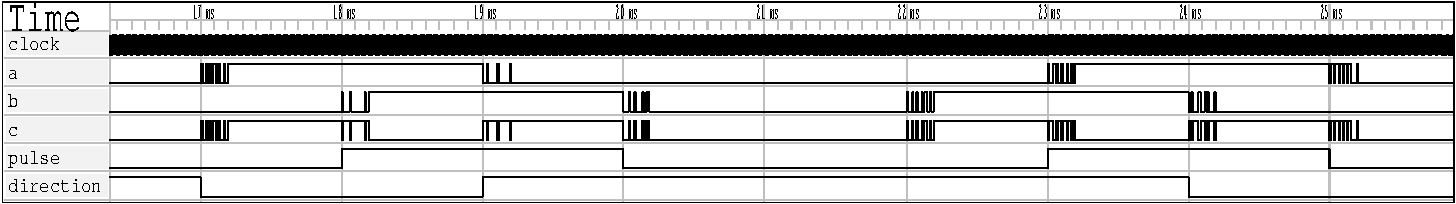
\includegraphics[width=\textwidth]{quadrature_decoder_gtkwave.pdf}
\caption{Waveforms of synchronous design}
\end{figure}
\begin{figure}
\centering
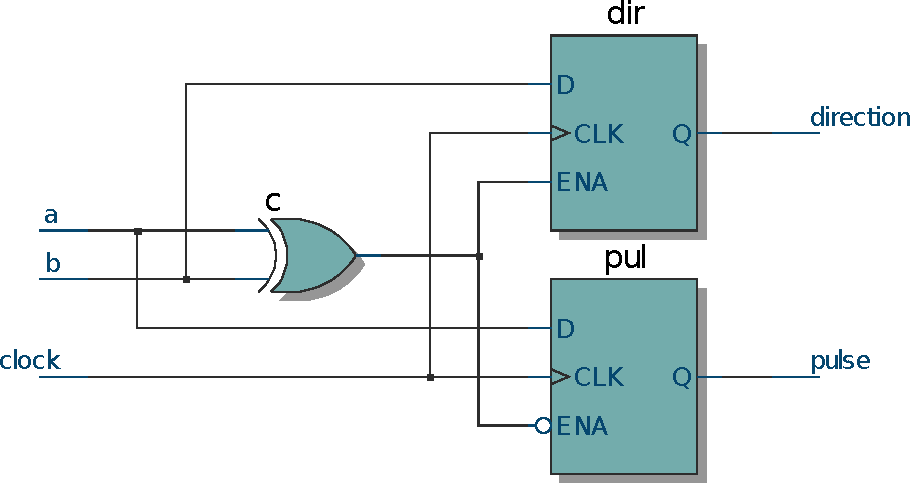
\includegraphics[width=0.5\textwidth]{quadrature_decoder_quartus_rtl.pdf}
\caption{RTL view of synchronous design}
\end{figure}
\begin{figure}
\centering
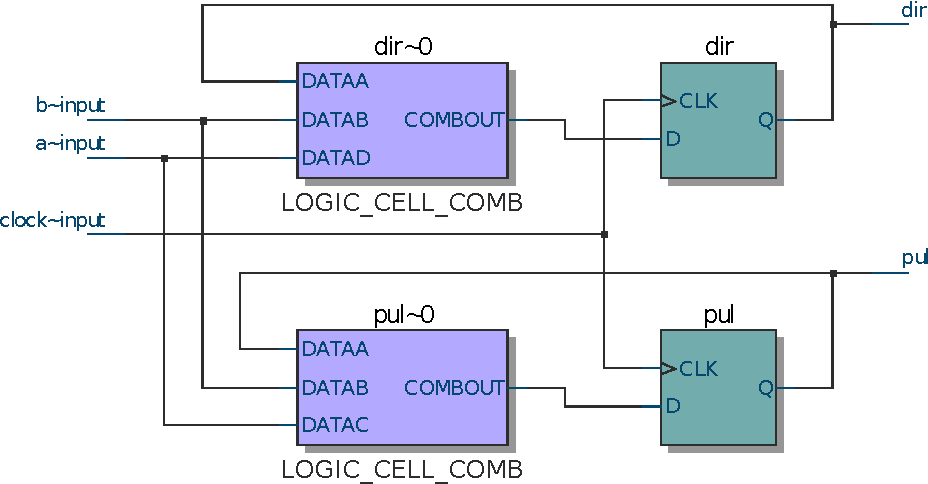
\includegraphics[width=0.5\textwidth]{quadrature_decoder_quartus_map.pdf}
\caption{Technology map view of synchronous design}
\end{figure}
\end{document}
